\section{Bias-tailoring II: repeating measurements}\label{sec:gauge_dcccs}

There is another technique we can use to tailor our code to certain noise biases, introduced in \Ccite{OscarSubsystemGaugeFixing}, where it was referred to as \textit{schedule-induced gauge-fixing} (SIGF) and applied to \textit{subsystem} codes.
In both subsystem codes and DCCCs, the check operators measured do not all mutually commute (these check operators are known as \textit{gauge operators} in a subsystem code or edge operators in DCCCs).
As a result, using a conventional measurement schedule, the measurement of each check operator is non-deterministic when considered in isolation, and must be combined with other (different) check operators to form a detector.

The SIGF method consists of \textit{repeating} the measurements of a mutually commuting subset of the check operators.
When a subset of mutually commuting gauge operators is measured, each check operator becomes an element of the ISG.
When the measurements of these check operators are repeated, the subsequent measurements are all deterministic (in the absence of noise), and so we can construct much smaller detectors formed from consecutive measurements of individual check operators.
Intuitively, by remaining in the same ISG while we repeat the commuting measurements, we can form much smaller detectors consisting of far fewer measurements, allowing us to protect against certain types of errors more effectively.
For example, if we remain in an ISG with detectors that protect more effectively against $Z$ errors, then this can be effective for handling $Z$-biased noise models (as was done in \Ccite{OscarSubsystemGaugeFixing}).

SIGF has been applied to subsystem codes \Ccite{OscarSubsystemGaugeFixing} and to the Floquet-Bacon-Shor codes \Ccite{SohaibAlam_2025}.
However, it has not previously been studied how well it can handle a noise model biased towards \textit{measurement} errors.
Intuitively we would expect SIGF to be advantageous in this setting, since each detector is formed from far fewer of the noisy measurements.
In this work, we apply SIGF to DCCCs.
Concretely, we simply repeat the edge operator measurements made at each timestep $t$ some number of times $r_t$.
We call the resulting new dynamical code a \textit{repeated DCCC} --
or, if we want to be specific, an \emph{$\mathbf{r}$-repeated DCCC}, where $\mathbf{r} = (r_0, r_1, \ldots)$.

In the next subsection we look analytically at how this intuition manifests itself in terms of detectors, logical errors and the decoding graph, and what we expect this to mean for the teraquop volumes.
Then we present numerical results and see how well our expectations hold up -- again, first for the more tractable case of direct parity measurement noise, and then the more realistic auxiliary qubit circuit noise.
Furthermore, we explore how repeated DCCCs perform both for $Z$ error bias and measurement bias.

\subsection{Detectors}\label{subsec:repeating_measurements_detectors}

Suppose a (unrepeated) DCCC has a detector
\begin{equation}\label{eq:unrepeated_detector}
    \prod_{(t \in \tau)}
        \prod_{(e_{\kappa_t} \in f_{\kappa})}
            m_t(\dcccOp{e}{\kappa_t}{P_t}),
\end{equation}
where $f_\kappa$ is the $\kappa$-coloured face to which the detector is associated,
and $\tau$ is a set of timesteps.
See, for example, the leftmost diagram of \Cref{fig:detector_if_measurements_done_twice}.
Now let $r_t \geq 1$ denote the number of times each measurement at timestep $t$ in the unrepeated DCCC is repeated before moving to the next measurement type,
let $R_t = \sum_{s=0}^{t-1} r_s$ be the total number of measurement rounds up to timestep $t$ in the unrepeated DCCC,
and for all $t \in \tau$ let $u_t$ be some integer in $\{0, \ldots, r_t-1\}$.
In the corresponding repeated DCCC, for each $\dcccOp{e}{\kappa_t}{P_t}$,
one can show that using the measurement outcomes $m_{R_t + u_t}(\dcccOp{e}{\kappa_{t}}{P_{t}})$ from
any timestep $R_t + u_t$ of each set of $r_t$ repeated measurement rounds gives a detector
\begin{equation}\label{eq:repeated_detector_using_first_round_measurements}
    \prod_{(t \in \tau)}
        \prod_{(e_{\kappa_{t}} \in f_{\kappa})}
            m_{R_t + u_t}(\dcccOp{e}{\kappa_{t}}{P_{t}}).
\end{equation}

\begin{figure}[tb]
    \centering
    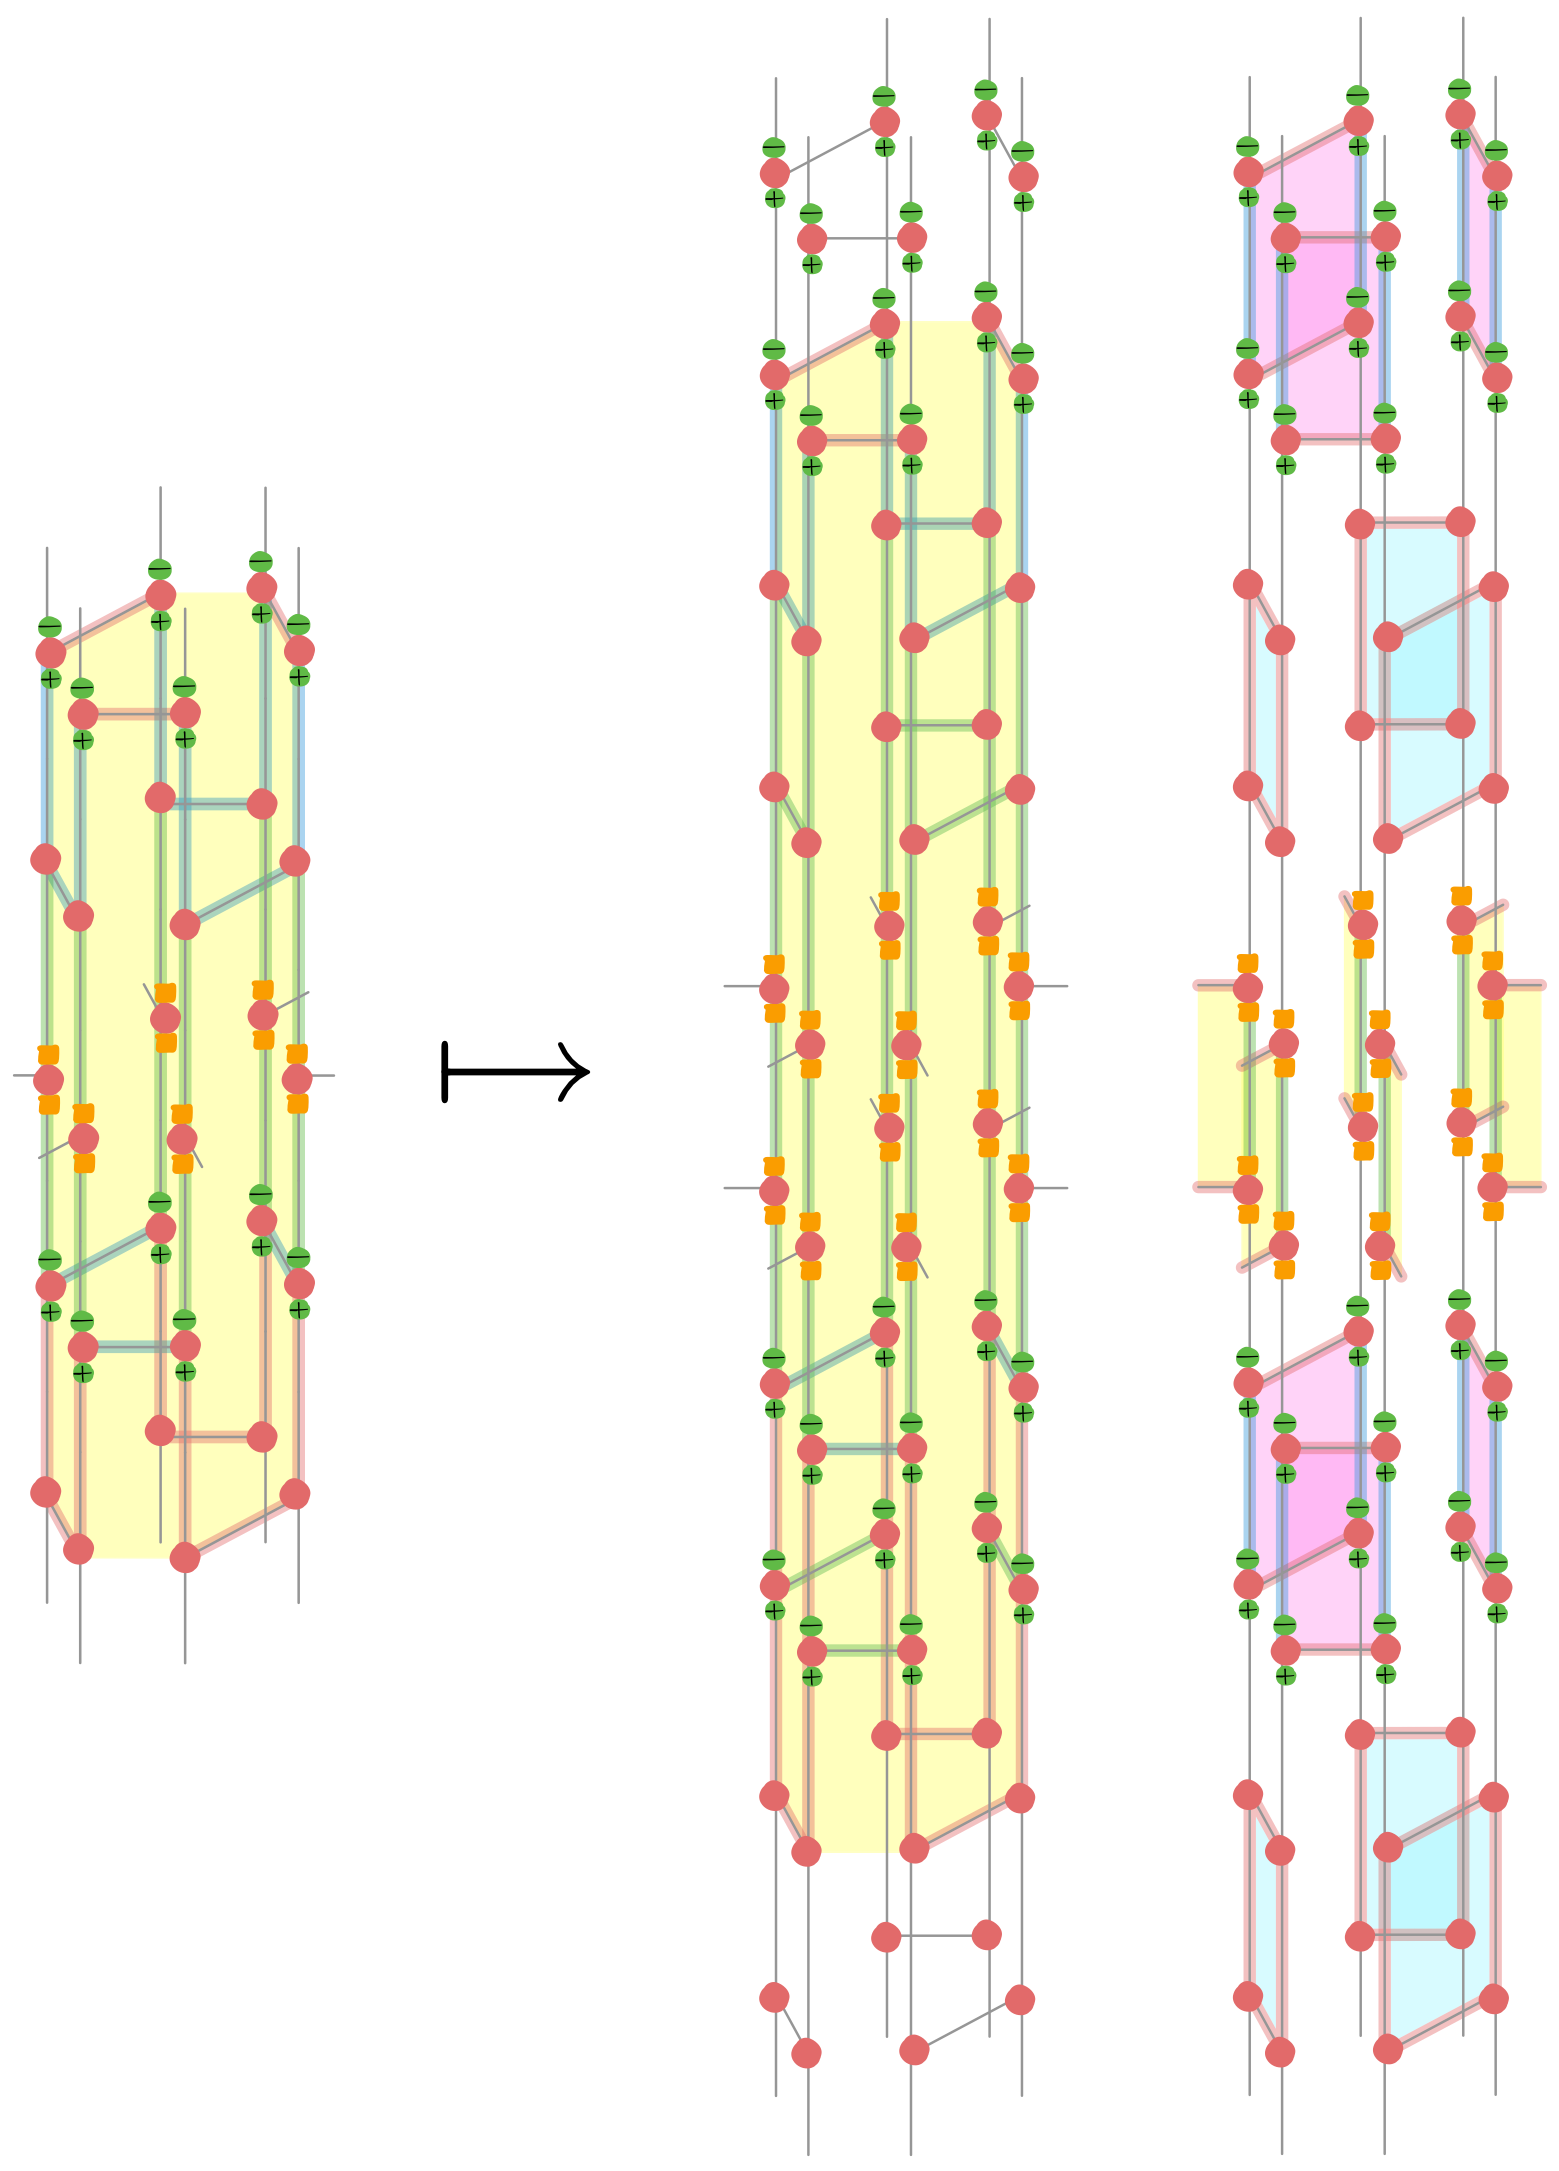
\includegraphics[width=0.6\linewidth]{figures/repeating_measurements/detector_if_measurements_done_twice}
    \caption{Left: a detector in the $X^1 Y^1 Z^1$ code with volume $6 \cdot 4 = 24$ consisting of 12 measurements (as can be read off from the Pauli web -- see \Cref{fig:detectors_XYZ_and_CSS}). Middle: the analogous detector in the repeated $X^2 Y^2 Z^2$ code, which now has volume $6 \cdot ((4-1) \cdot 2 + 1) = 42$ but still consists of 12 measurements. Right: the edge detectors on these six qubits in the $X^2 Y^2 Z^2$ code, each of which has volume 2 and consists of two consecutive edge measurements.
    As discussed more in the caption of \Cref{tab:repeated_xyz_css_averages}, repeating measurements reduces the mean detector volume and measurements per detector, while increasing the mean number of detectors per measurement -- all of which our intuition says are improvements.
    On the other hand, it increases the maximum detector volume.
    In any case, our simulations show that these improvements don't generally outweigh the negative effects of repeating measurements, except in the case of high measurement bias.}
    \label{fig:detector_if_measurements_done_twice}
\end{figure}

We show an example of such a detector in the middle diagram of \Cref{fig:detector_if_measurements_done_twice}, with $r_t = 2$ for all $t$.
However, some choices of $u_t$ are more sensible than others.
Firstly, we want the detector to span as few timesteps as possible;
this minimises the probability of the detector being violated,
which makes the job of the decoder easier, as discussed earlier.
Secondly, we still want to be able to use a matching decoder.

Letting $T = \max(\tau)$ be the latest timestep in $\tau$,
we can achieve these two conditions by
using measurements from the final round $R_t + r_t-1$ of $r_t$ repeated measurement rounds for all $t \neq T$,
but using measurements from the first round $R_T$ of $r_T$ repeated measurements rounds for $t = T$
\begin{equation}\label{eq:repeated_detector_sensible}
    \prod_{(t \in \tau - \{T\})}
        \prod_{(e_{\kappa_{t}} \in f_{\kappa})}
            m_{R_t + r_t-1}(\dcccOp{e}{\kappa_{t}}{P_{t}})
    \prod_{(e_{\kappa_{T}} \in f_{\kappa})}
        m_{R_T}(\dcccOp{e}{\kappa_{T}}{P_{T}}).
\end{equation}

Indeed, this is the specific choice of measurements used in the example in \Cref{fig:detector_if_measurements_done_twice}.
In this new repeated DCCC,
we also have detectors with no analogue to any of those in the original DCCC.
Suppose we have just measured all $(\kappa, P)$ edge operators at some timestep $R_t$
for the first of $r_t$ repeated measurement rounds.
Each edge operator $\dcccOp{e}{\kappa}{P}$ is therefore now a stabilizer up to some sign $m_{R_t}(\dcccOp{e}{\kappa}{P})$.
Assuming $r_t > 1$, at the next timestep $R_t + 1$ we measure all these $(\kappa, P)$ edge operators again.
The stabilizer formalism says that each such measurement will give us the deterministic outcome
$m_{R_t+1}(\dcccOp{e}{\kappa}{P}) = m_{R_t}(\dcccOp{e}{\kappa}{P})$ in the absence of any noise,
so the formal product $m_{R_t+1}(\dcccOp{e}{\kappa}{P}) m_{R_t}(\dcccOp{e}{\kappa}{P})$ is a detector,
for all $\kappa$-coloured edges $e_{\kappa}$.
Indeed, we get two-measurement detectors like these at every subsequent timestep
in the set of $r_t$ repeated measurement rounds.
That is, for every $u \in \{1, \ldots, r_t-1\}$,
we get a detector $m_{R_t + u}(\dcccOp{e}{\kappa}{P}) m_{R_t + u-1}(\dcccOp{e}{\kappa}{P})$
for all $\kappa$-coloured edges $e_{\kappa}$.
These are shown in the rightmost diagram in \Cref{fig:detector_if_measurements_done_twice}.
Since each such detector is associated to an edge, we call them \textit{edge detectors},
and will refer to the other type of detectors (those associated to a face) as \textit{face detectors}.\subsubsection{Volume, measurements per detector, detectors per measurement}\label{subsubsec:repeating_measurements_volume_measurements_detectors}

Let's now contrast these new detectors in the repeated DCCC with those of the corresponding unrepeated DCCC.
First note the number of timesteps spanned by a face detector in the repeated DCCC is at least as large as in the unrepeated DCCC.
Indeed, a face detector in an unrepeated DCCC whose first measurements were at timestep $t$ and final measurements were at timestep $T$, and thus spanned $T - t$ timesteps, will now span $R_T - (R_t + r_t - 1)$ timesteps.
If any $r_j > 1$ for $j \in \{t+1, \ldots, T-1\}$ then this is larger than $T-t$.
We'll define the \textit{volume} of a detector in a DCCC\footnote{Not to be confused with the teraquop volume of the DCCC as a whole! Also, as noted in a previous footnote, a more accurate metric capturing the same intuition is detector likelihood \cite{hesner2024using}.} as the product of the number of timesteps it spans and the number of data qubits involved in the measurements that make up this detector.
Intuitively, the smaller the volume, the better, because a smaller volume means there are fewer opportunities for this detector to be violated.
For example, the detectors in the unrepeated $X^1 Y^1 Z^1$ and $X^1 Z^1$ codes all have volume $6 \cdot 4 = 24$ (\Cref{fig:detectors_XYZ_and_CSS}).
In a repeated version with $r_t$ set to some $r$ for all $t$, these detectors would have volume $6 \cdot ((4-1)r + 1)$ (\Cref{fig:detector_if_measurements_done_twice}).

On the other hand, the number of measurements per face detector remains exactly the same -- e.g.\ $12$ for any $\mathbf{r}$-repeated $X^a Y^b Z^c$ code, and 6 for any $\mathbf{r}$-repeated $X^a Z^b$ code.
Thanks to the new edge detectors, however, which always have volume two and consist of two measurements, the \emph{average} detector volume and \emph{average} number of measurements per detector decreases.
Indeed, in the limit where $r_t \to \infty$ for all $t$, the edge detectors dominate, and these averages both tend to two.
For our two favourite DCCCs, we compute these averages exactly in \Cref{tab:repeated_xyz_css_averages}.

\begin{difference}\label{dif:repeating_detectors}
    Repeating measurements increases the maximum detector volume of a DCCC,
    while decreasing its minimum detector volume and minimum measurements per detector.
    Overall, it decreases a DCCC's average detector volume and average number of measurements per detector.
\end{difference}

Intuitively, smaller volumes and fewer measurements per detector are better, so the fact these averages decrease might suggest a general performance improvement.
However, there is an important trade-off: while the new edge detectors catch measurement errors quickly (with volume 2), data qubit errors can accumulate for longer before being detected.

\begingroup
\renewcommand*{\arraystretch}{1.5}
\begin{table}[tb]
    \centering
    \begin{tabular}{|c|c|c|c|}
        \hline
        & & $X^r Y^r Z^r$ & $X^r Z^r$ \\
        \hline
        \multirow{3}{*}{Detector volume} & Max & $6 \cdot (3r + 1) \to \infty$ & $6 \cdot (3r + 1) \to \infty$ \\
        \cline{2-4}
        & Min & $2$ & $2$ \\
        \cline{2-4}
        & Average & $2 + \frac{22}{3r - 2} \to 2$ & $2 + \frac{22}{3r - 2} \to 2$ \\
        \hline
        \multirow{3}{*}{Meas.\ per detector} & Max & $12$ & $6$ \\
        \cline{2-4}
        & Min & $2$ & $2$ \\
        \cline{2-4}
        & Average & $2 + \frac{10}{3r - 2} \to 2$ & $2 + \frac{4}{3r - 2} \to 2$ \\
        \hline
        \multirow{3}{*}{Detector degree} & Max & $12 + 6(r-1) \to \infty$ & $12 + 6(r-1) \to \infty$ \\
        \cline{2-4}
        & Min & $4$ & $4$ \\
        \cline{2-4}
        & Average & $6 + \frac{6}{3r - 2} \to 6$ & $6 + \frac{6}{3r - 2} \to 6$ \\
        \hline
    \end{tabular}
    \caption{
        Comparison of metrics concerning detectors in the $X^r Y^r Z^r$ and $X^r Z^r$ codes, for $r > 1$.
        The arrows denote the limit of an expression as $r$ tends to infinity.
        As described in \Cref{dif:repeating_detectors}, repeating measurements increases a DCCC's max.\ detector volume while decreasing its min.\ detector volume and min.\ measurements per detector.
        Overall, it decreases a DCCC's average detector volume and average number of measurements per detector.
        Intuitively smaller volumes and fewer measurements per detector are better,
        so the fact these averages decrease might suggest a general performance improvement.
        On the other hand, the key metric could be the maximum or minimum over all these values.
    }
    \label{tab:repeated_xyz_css_averages}
\end{table}
\endgroup

\subsubsection{Asymmetric schedules}\label{subsubsec:repeating_measurements_asymmetric_schedules}

By using asymmetric schedules (where $r_t$ is not the same for all $t$), we can try to further tailor our code to $Z$-biased noise models.
Here the intuition is that if physical $Z$ errors are more likely to occur, we can spend more time measuring $\dcccOp{e}{\kappa}{X}$ and $\dcccOp{e}{\kappa}{Y}$ operators, which will create more edge detectors that are violated by Pauli $Z$ errors.
The more of these we have, the more accurately we can detect and correct Pauli $Z$ errors.

For example, consider the $X^a Z^b$ code, where we repeat all $\dcccOp{e}{\kappa}{X}$ operators $a$ times
and all $\dcccOp{e}{\kappa}{Z}$ operators $b$ times.
In a $Z$-biased noise model, we expect that setting $a$ to be larger than $b$ improves performance.
Similarly, consider the $X^a Y^b Z^c$ code, suppose we repeat all $\dcccOp{e}{\kappa}{X}$ operators $a$ times, all $\dcccOp{e}{\kappa}{Y}$ operators $b$ times, and all $\dcccOp{e}{\kappa}{Z}$ operators $c$ times.
Here we expect that setting $a$ and $b$ to be larger than $c$ will improve performance.

\begin{difference}\label{dif:repeating_asymmetric_schedule}
    In a repeated DCCC, we can choose to spend more time measuring operators that will form detectors capable of detecting certain types of Pauli errors.
    This is particularly relevant for $Z$-biased noise models.
\end{difference}

%We can track all of this via the boson grid.
%Suppose at times $tr, \ldots, tr + r - 1$ we repeatedly measure all $(c, P)$ edge operators,
%before swapping to measuring all $(c', P')$ edge operators at time $(t+1)r$.
%Then, up to $\pm 1$ signs, we have:
%\begin{equation}\label{eq:gauge_DCCC_new_groups}
%\begin{gathered}
%    \begin{aligned}
%        \SSS_{tr} &= \ldots &&= \SSS_{tr + r - 2} &&= \SSS_{tr + r - 1}
%        &&= \groupPres{\ \scalebox{0.7}{\bosonTable{
%            condensed = rx,
%            rowLabel = e,
%            columnLabel = m,
%            rx = {\filledHexagon \diagup},
%            gz = {\filledHexagon},
%            bz = {\filledHexagon},
%        }}\ }\\[5pt]
%        \DDD_{tr} &= \ldots &&= \DDD_{tr + r - 2}
%        &&&&= \groupPres{\ \scalebox{0.7}{\bosonTable{
%            condensed = rx,
%            rowLabel = e,
%            columnLabel = m,
%            rx = {\filledHexagon \diagup},
%            gz = {\filledHexagon},
%            bz = {\filledHexagon},
%        }}\ }\\[5pt]
%        &&&&&\DDD_{tr + r - 1} &&= \groupPres{\ \scalebox{0.7}{\bosonTable{
%            condensed = rx,
%            rowLabel = e,
%            columnLabel = m,
%            rx = {\filledHexagon},
%            gy = {\filledHexagon},
%            bx = {\filledHexagon},
%            by = {\filledHexagon},
%        }}\ }\\[5pt]
%        \LLL_{tr} &= \ldots &&= \LLL_{tr + r - 2} &&= \LLL_{tr + r - 1}
%        &&= \groupPres{
%            \ol{i},
%            \ol{x_{1, tr}},
%            \ol{z_{1, tr}},
%            \ol{x_{2, tr}},
%            \ol{z_{2, tr}}}
%    \end{aligned}\\[5pt]
%    \text{where }
%    x_{1, tr} \in \pm\ \scalebox{0.5}{\bosonTable{
%        condensed = rx,
%        rowLabel = e,
%        columnLabel = m,
%        gx={\rightarrow},
%    }},\
%    z_{1, tr} \in \pm\ \scalebox{0.5}{\bosonTable{
%        condensed = rx,
%        rowLabel = e,
%        columnLabel = m,
%        ry={\uparrow},
%    }},\
%    x_{2, tr} \in \pm\ \scalebox{0.5}{\bosonTable{
%        condensed = rx,
%        rowLabel = e,
%        columnLabel = m,
%        gx={\uparrow},
%    }},\
%    z_{2, tr} \in \pm\ \scalebox{0.5}{\bosonTable{
%        condensed = rx,
%        rowLabel = e,
%        columnLabel = m,
%        ry={\rightarrow},
%    }}
%\end{gathered}
%\end{equation}
%%The  Immediately after the remaining timestep $tr + r - 1$, up to $\pm 1$ signs, we have:
%%\begin{equation}\label{eq:gauge_DCCC_tr-1_groups}
%%    \begin{gathered}
%%        \begin{aligned}
%%            \SSS_{tr + r - 1} &= \groupPres{\ \scalebox{0.7}{\bosonTable{
%%                condensed = rx,
%%                rowLabel = e,
%%                columnLabel = m,
%%                rx = {\filledHexagon \diagup},
%%                gy = {\filledHexagon},
%%                by = {\filledHexagon},
%%            }}\ }\\[5pt]
%%            \DDD_{tr + r - 1} &= \groupPres{\ \scalebox{0.7}{\bosonTable{
%%                condensed = rx,
%%                rowLabel = e,
%%                columnLabel = m,
%%                rx = {\filledHexagon},
%%                gy = {\filledHexagon},
%%                bx = {\filledHexagon},
%%                by = {\filledHexagon},
%%            }}\ }\\[5pt]
%%            \LLL_{tr + r - 1} &= \groupPres{
%%                \ol{i},
%%                \ol{x_{1, tr + r - 1}},
%%                \ol{z_{1, tr + r - 1}},
%%                \ol{x_{2, tr + r - 1}},
%%                \ol{z_{2, tr + r - 1}}}
%%        \end{aligned}\\[5pt]
%%%        \text{where }
%%        x_{1, tr + r - 1} \in \pm\ \scalebox{0.5}{\bosonTable{
%%            condensed = rx,
%%            rowLabel = e,
%%            columnLabel = m,
%%            gx={\rightarrow},
%%        }},\
%%        z_{1, tr + r - 1} \in \pm\ \scalebox{0.5}{\bosonTable{
%%            condensed = rx,
%%            rowLabel = e,
%%            columnLabel = m,
%%            ry={\uparrow},
%%        }},\
%%        x_{2, tr + r - 1} \in \pm\ \scalebox{0.5}{\bosonTable{
%%            condensed = rx,
%%            rowLabel = e,
%%            columnLabel = m,
%%            gx={\uparrow},
%%        }},\
%%        z_{2, tr + r - 1} \in \pm\ \scalebox{0.5}{\bosonTable{
%%            condensed = rx,
%%            rowLabel = e,
%%            columnLabel = m,
%%            ry={\rightarrow},
%%        }}
%%    \end{gathered}
%%\end{equation}

\subsection{Logical errors}\label{subsec:repeating_measurements_logical_errors}

\begin{figure}[htbp]
    \centering
    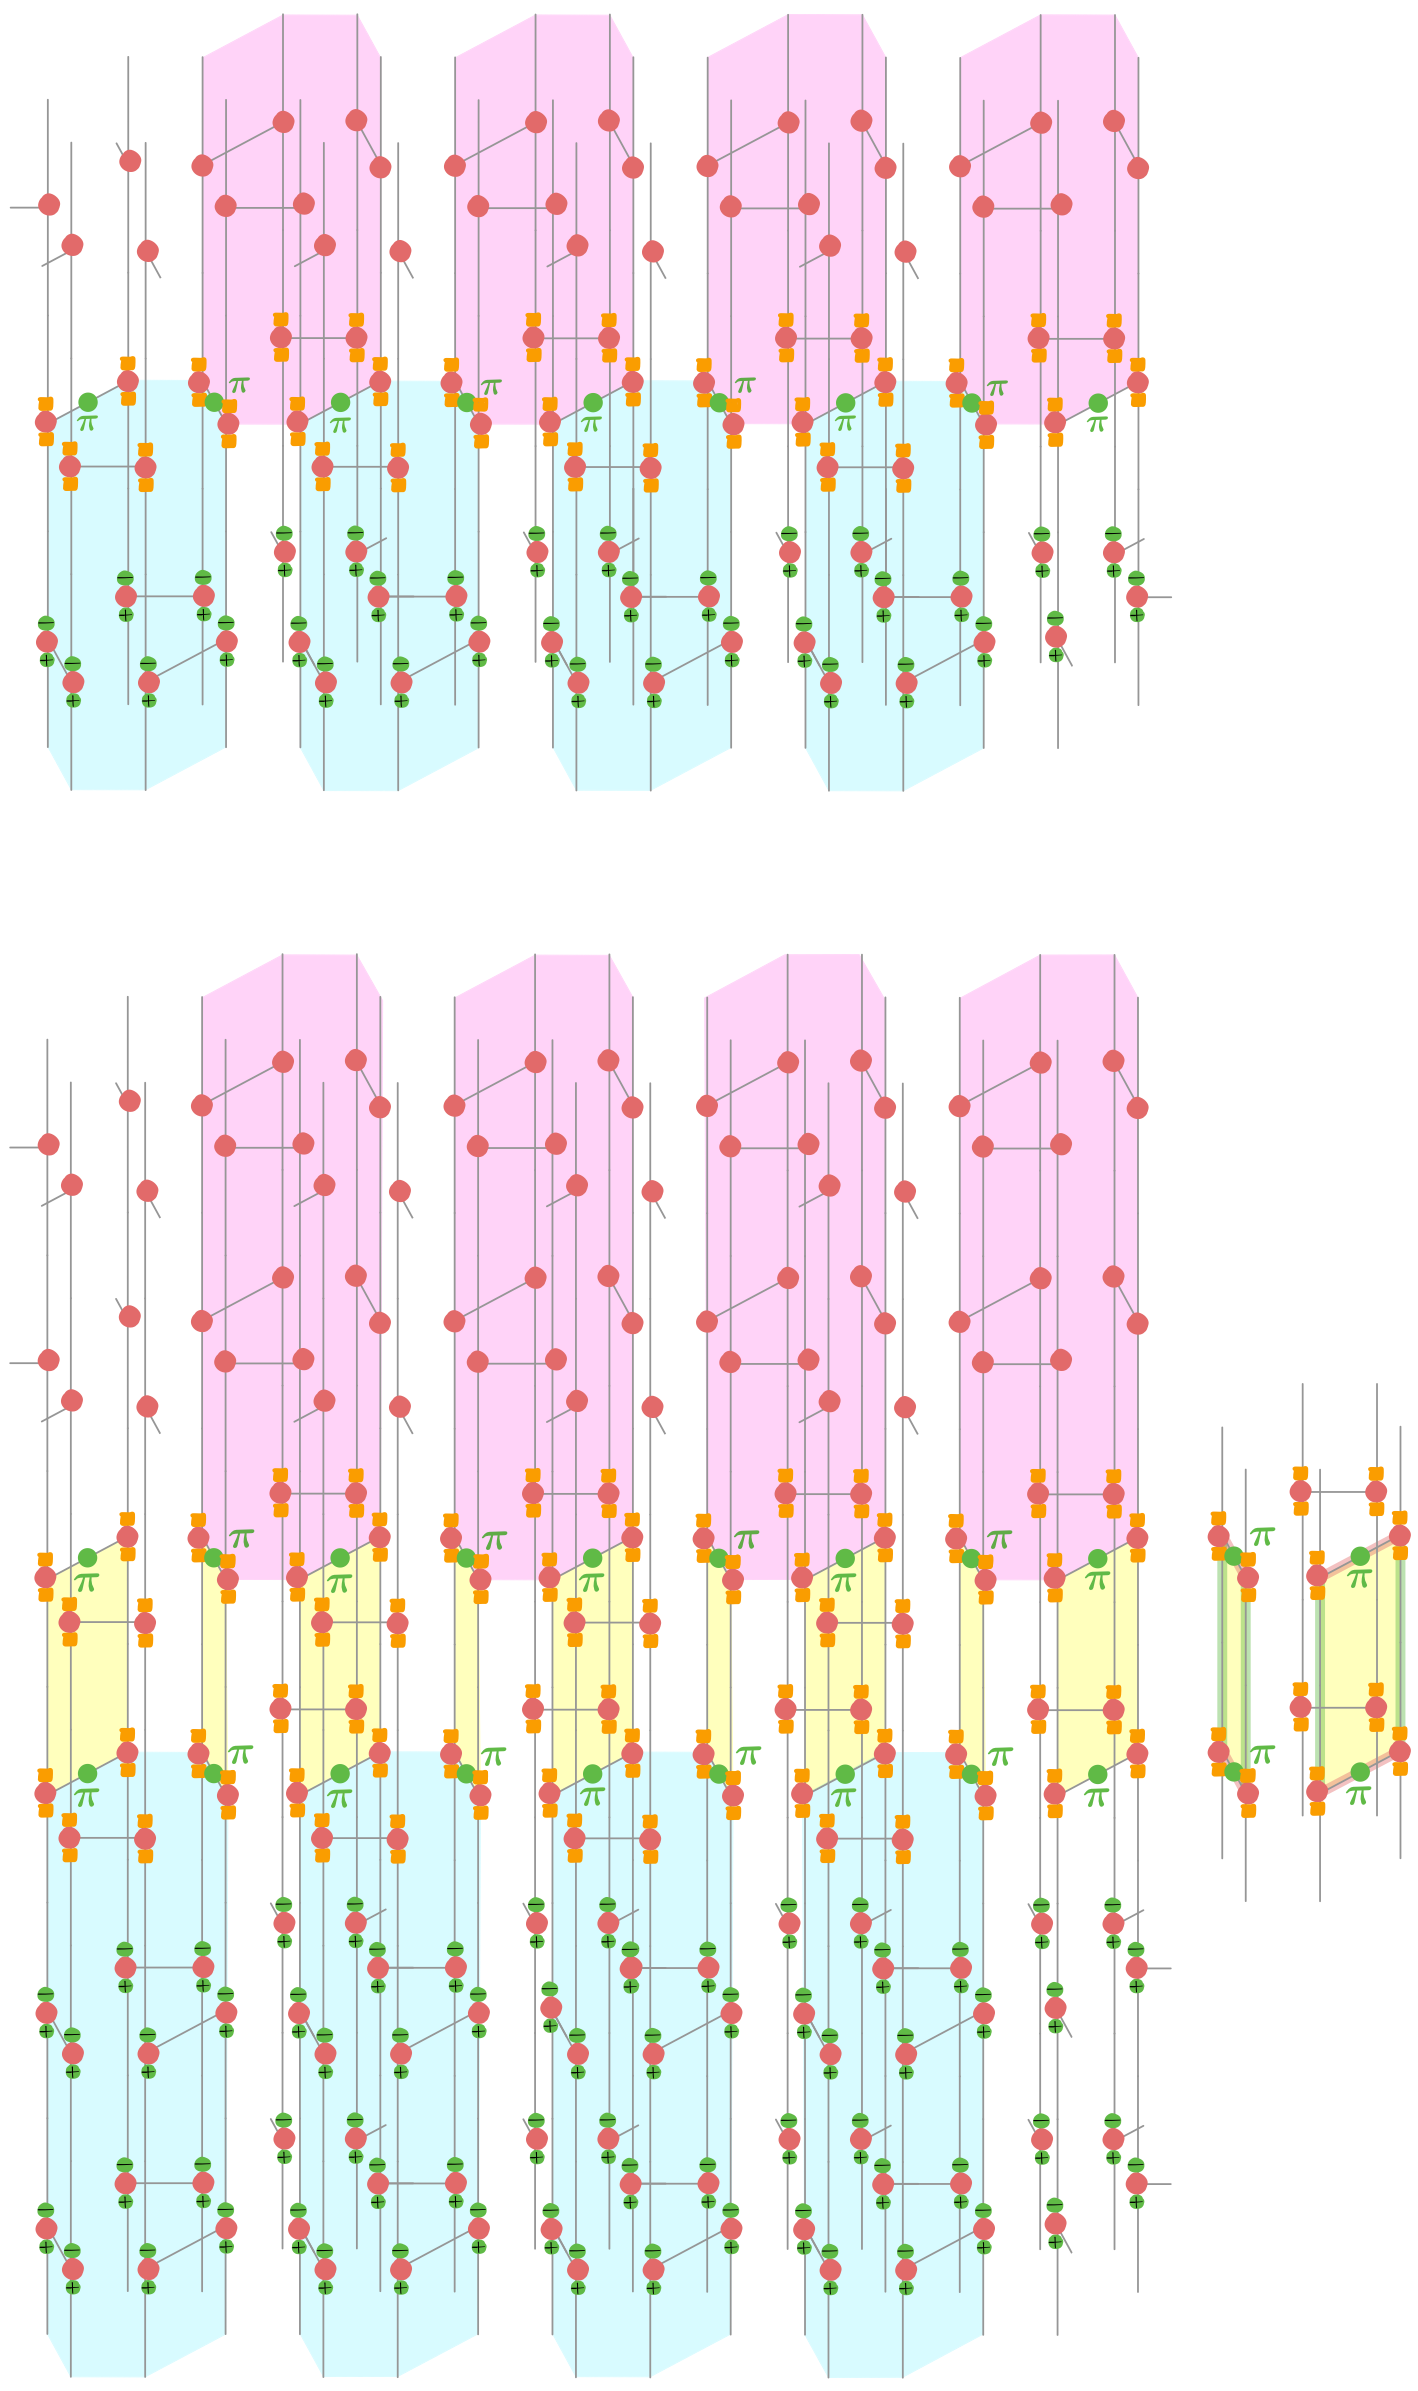
\includegraphics[height=0.77\textheight]{figures/repeating_measurements/spacelike_logical_from_measurement_errors_repeated_DCCC}
        \caption{
            Top: a spacelike logical error in the $X^1 Y^1 Z^1$ code consisting entirely of measurement errors.
            Bottom: the analogous spacelike logical error in the $X^2 Y^2 Z^2$ code.
            This again consists entirely of measurement errors, but there are twice as many of them as before, because of the addition of the yellow edge detectors in the $X^2 Y^2 Z^2$ code.
            In both diagrams we only show one type ($E$ or $M$) of detectors.
            We draw the Pauli webs for two edge detectors to show that the logical error really doesn't violate any detectors (see \Cref{fig:XYZ_measurement_error} or \Cref{sec:zx-calculus-and-pauli-webs}),
            but otherwise omit the Pauli webs -- they can be found in \Cref{sec:detectors-cheatsheet}.
            There is a bijection between spacelike logical errors consisting entirely of measurement errors in the $X^1 Y^1 Z^1$ code and in any $X^a Y^b Z^c$ code.
            Hence repeating measurements in general increases the spacelike distance with respect to pure measurement noise (\Cref{tab:repeated_xyz_css_distances}).
            One might then expect this to improve the teraquop width $\tilde{n}_{E}$ and length $\tilde{n}_M$,
            especially in more measurement-biased noise models (\Cref{dif:repeated_spacelike_logicals}).
            But the simulations don't seem to back this up (\Cref{fig:X1Z1_X3Z3_comparison}).
        }
    \label{fig:spacelike_logical_from_measurement_errors_repeated_DCCC}
\end{figure}

\begin{figure}[htbp]
    \centering
    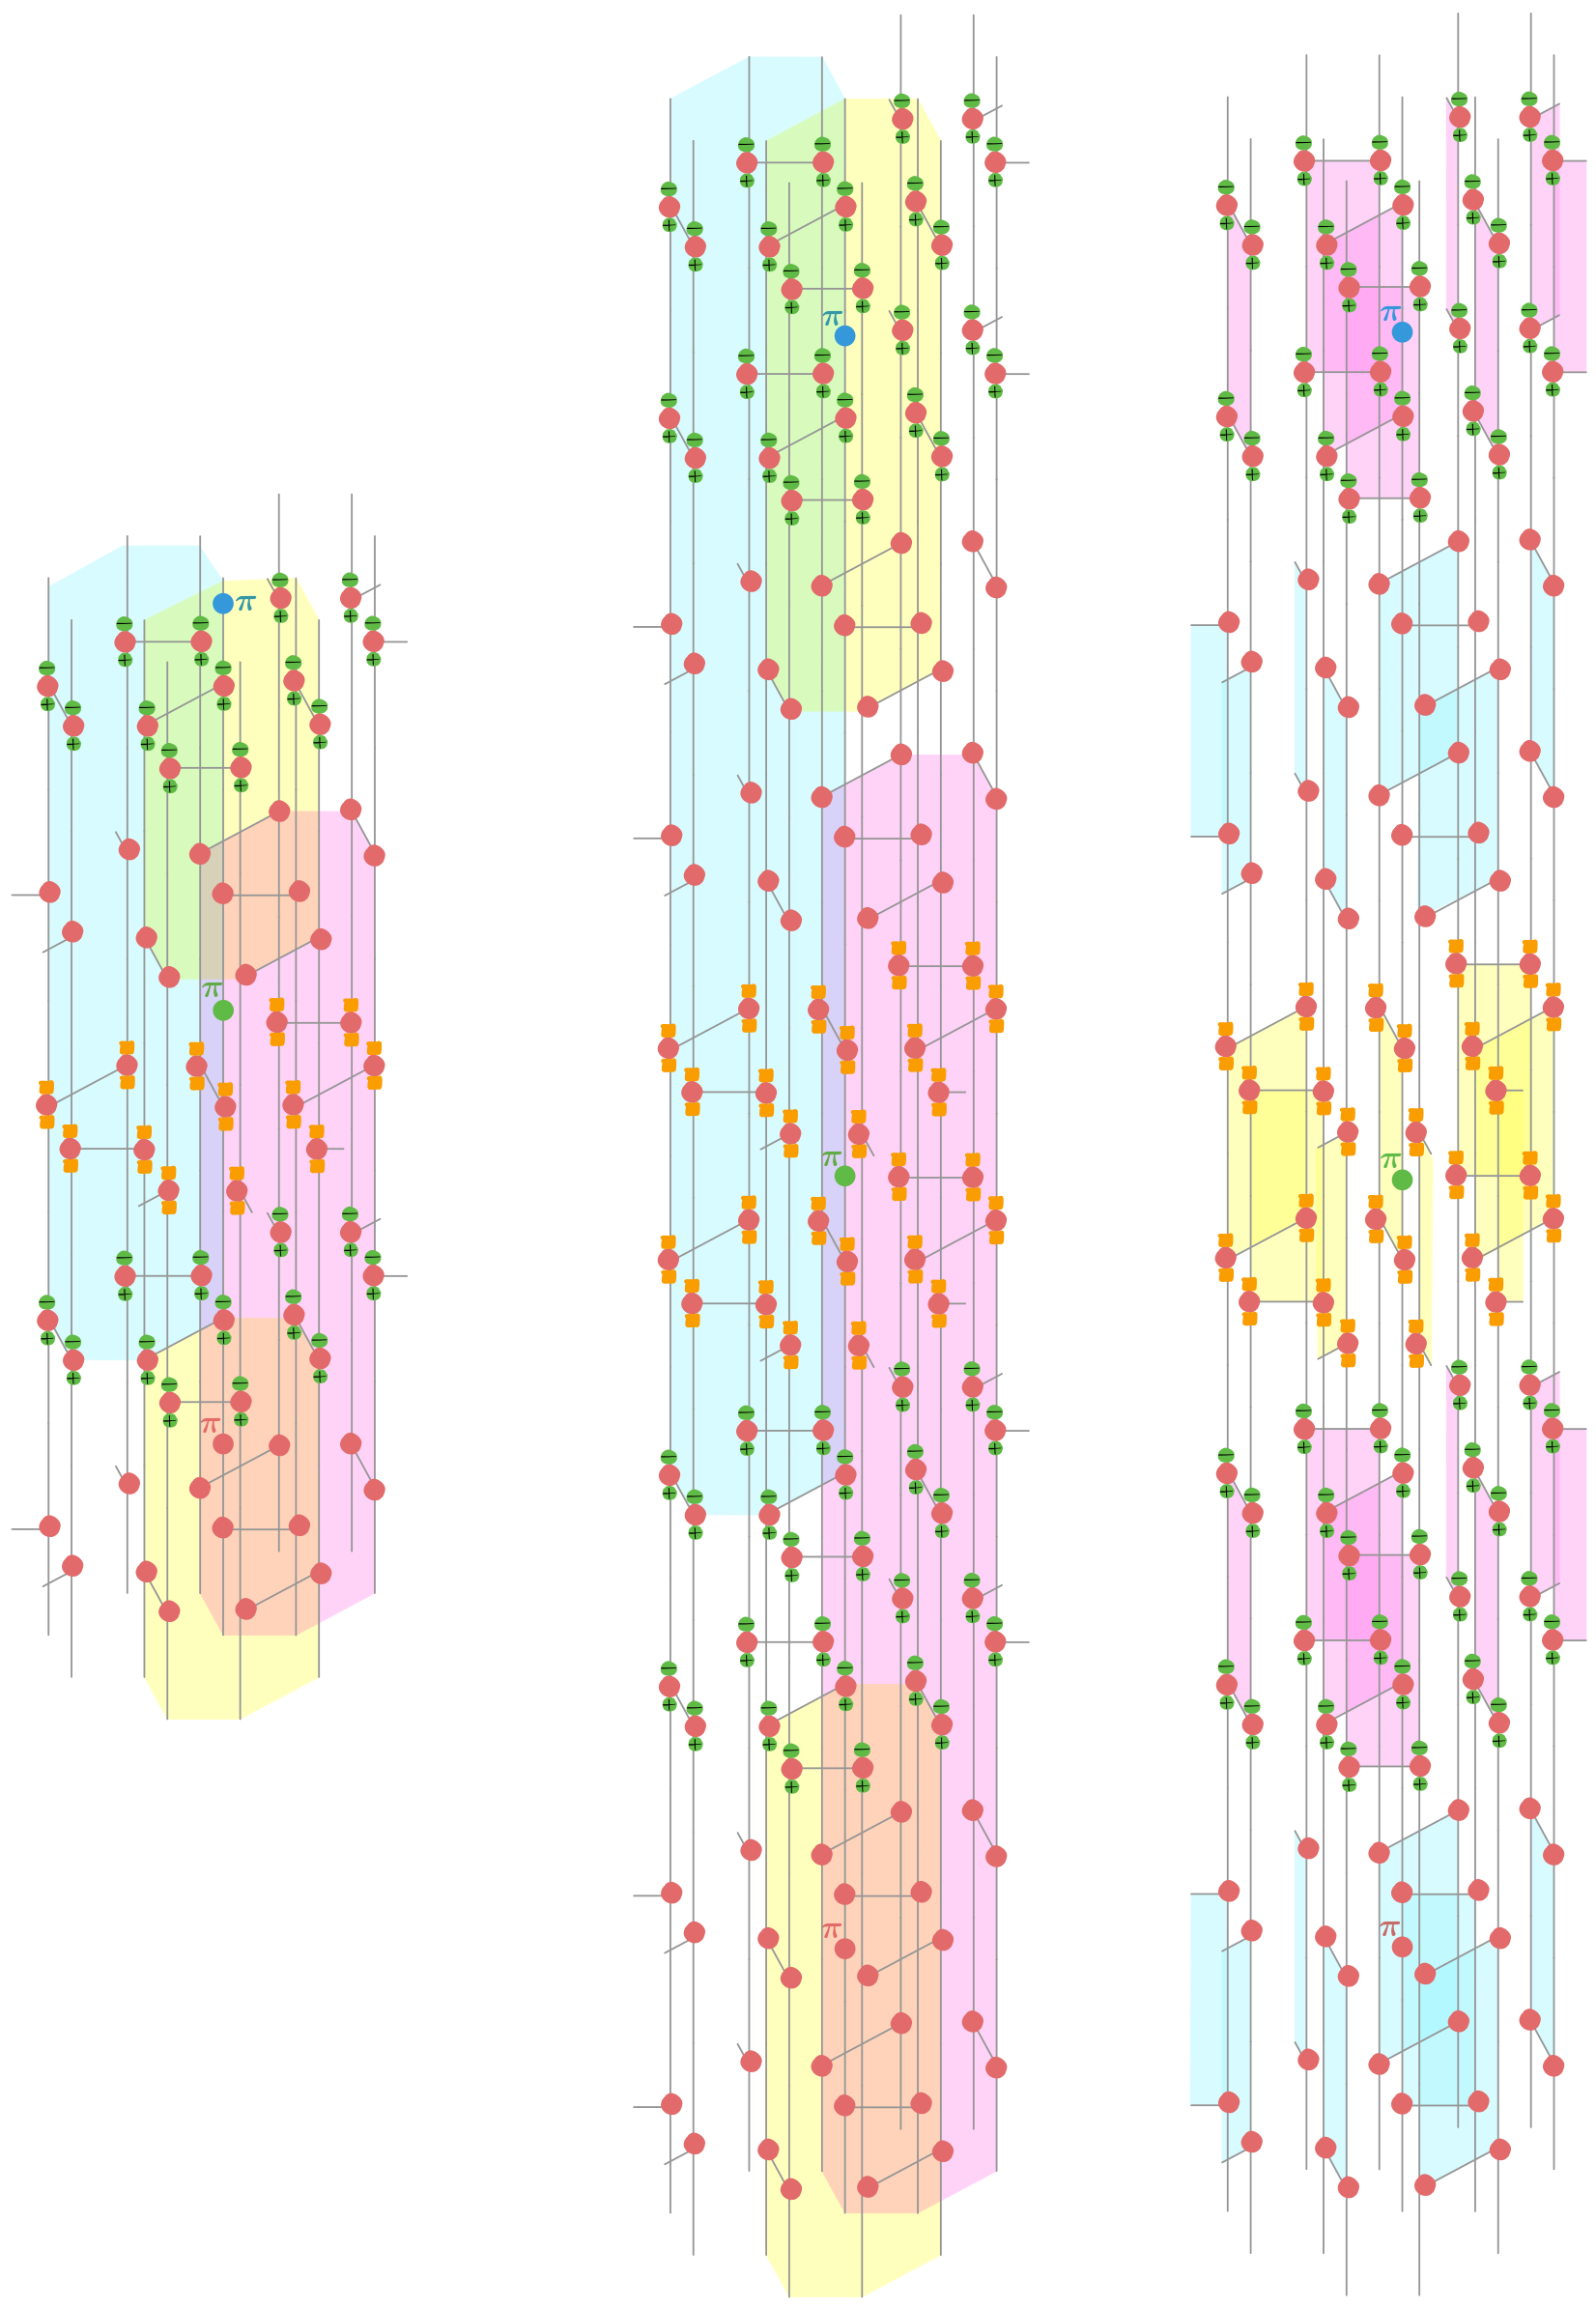
\includegraphics[height=0.75\textheight]{figures/repeating_measurements/timelike_logical_from_data_qubit_errors_repeated_DCCC}
    \caption{
        Left: a subset of a timelike logical error in the $X^1 Y^1 Z^1$ code consisting entirely of data qubit errors.
        Middle: the analogous timelike logical error in the $X^2 Y^2 Z^2$ code, with half ($E$ or $M$) of the face detectors indicated.
        Right: the same logical error but with the edge detectors indicated.
        In all diagrams, the Pauli webs are omitted -- they can be found in \Cref{sec:detectors-cheatsheet}.
        The logical error in the $X^2 Y^2 Z^2$ code in the middle and right subfigures again consists entirely of data qubit errors, but these data qubit errors now occur once every four rounds rather than once every two rounds.
        In other words, if these two codes were implemented for the same number of rounds, the logical in the $X^2 Y^2 Z^2$ code would have half the weight of the one in the $X^1 Y^1 Z^1$ code.
        Indeed, repeating measurements in general decreases the timelike distance with respect to pure data qubit noise (\Cref{tab:repeated_xyz_css_distances}).
        One would then expect this to worsen the teraquop heights $\tilde{h}_{E}$ and $\tilde{h}_M$,
        especially in more $Z$-biased noise models (\Cref{dif:repeated_timelike_logicals}).
        While the simulation results do show this to be the case (\Cref{fig:X1Z1_X3Z3_comparison}), the fact that this difference is greatest for unbiased noise rather than $Z$-biased noise suggests its cause is something more than the reason discussed here.
    }
    \label{fig:timelike_logical_from_data_qubit_errors_repeated_DCCC}
\end{figure}

The $(n_M, m_E, h_\mathbf{r})$-block definition from \Cref{subsec:estimating-teraquop-volume} still makes sense for any $\mathbf{r}$-repeated DCCC;
we just write $h_{\mathbf{r}}$ instead of $h$ to make it clear that we're considering a repeated DCCC.
%Likewise we can again consider $(s_X, s_Z, h_{\mathbf{r}})_X$- and $(s_X, s_Z, h_{\mathbf{r}})_Z$-blocks.
% as defined above, but with the measurement of edge operators $\dcccOp{E}{\kappa_t}{P_t}$ at timestep $t$ repeated $r_t$ times.
Repeating measurements can increase our code's resilience against spacelike logical errors consisting only of measurement errors.
Consider such a logical error in the unrepeated DCCC, consisting of measurement errors on a set of edge operators $\{\dcccOp{e}{\kappa}{P}\}$ all occurring at the timestep $t$.
For every error in this set,
consider an error on the measurement of $\dcccOp{e}{\kappa}{P}$ at \emph{all} $r_t$ repeated timesteps $R_t + u_t$ for $u_t \in \{0, \ldots, r_t - 1\}$.
The union of all such errors forms a spacelike logical error in the repeated DCCC.
The key here is that each new edge detector
$m_{R_t + u_t}(\dcccOp{e}{\kappa}{P}) m_{R_t + u_t - 1}(\dcccOp{e}{\kappa}{P})$
would be violated by a measurement error on $\dcccOp{e}{\kappa}{P}$ at timestep $R_t + u_t$ or $R_t + u_t - 1$.
So in order for no such detector to be violated, we need the measurements at both timesteps to be erroneous, thereby cancelling each other out.
All pure measurement noise spacelike errors in the repeated DCCC are formed in this way.
So the spacelike distance with respect to these types of logical errors specifically is $(\min_{t} r_t) \cdot d_s$.
An example is shown in \Cref{fig:spacelike_logical_from_measurement_errors_repeated_DCCC}.
% This provides more evidence that repeating measurements is a good idea, especially if the noise is biased towards measurement errors.

\begin{difference}\label{dif:repeated_spacelike_logicals}
    Repeating measurements increases a DCCC's resilience against spacelike logical errors consisting entirely of measurement errors.
    This is particularly relevant in measurement biased noise models.
\end{difference}

On the other hand, repeating measurements generally decreases a DCCC's resilience against timelike logical errors consisting only of data qubit errors.
Again, all such logical errors are analogues of those in the unrepeated DCCC.
Consider such an error in the unrepeated DCCC.
For every Pauli $P$ data qubit error on qubit $j$ immediately after timestep $t$ in the unrepeated DCCC,
the analogous logical error in the repeated DCCC consists of a Pauli $P$ error on qubit $j$ at \emph{any} timestep $R_t + u_t$ for $u_t \in \{0, \ldots, r_t - 1\}$.
Letting $\tau$ again be the set of timesteps of the measurement errors in the unrepeated DCCC,
where before the logical error consisted of $|\tau|$ errors across $h$ timesteps,
it's now $|\tau|$ across $h_{\mathbf{r}} = \sum_{0 < t < h} r_t$.
As soon as $r_t > 1$ for some $t$, this is a decrease.
% That is, in order to maintain the same timelike distance, we have to use block height $h_{\mathbf{r}} = \sum_{0 < t < h} r_t \geq h$.
%Reaching again for the example of an $(s_X, s_Z, h)_X$ block of CSS honeycomb code,
For example, in an $(n_M, n_E, h)$ block of the $X^1 Y^1 Z^1$ code,
in which there exist timelike logical errors consisting of a data qubit error every 2 rounds.
Now suppose we repeat all measurements some fixed number of times $r > 1$ to get an $(n_M, n_E, h_{\mathbf{r}})$ block of the $X^r Y^r Z^r$ code.
Under pure data qubit noise, the unrepeated code has a timelike distance of $\frac{h}{2}$,
whereas the repeated code has a (worse) timelike distance of $\frac{h_{\mathbf{r}}}{2r}$.
See \Cref{fig:timelike_logical_from_data_qubit_errors_repeated_DCCC}.

% Alternatively, as in the last subsection, we could have chosen to repeat all $XX$ measurements $r_X$ times,
% and all $ZZ$ measurements $r_Z$ times.
% Note that $X$ data qubit errors can only contribute to timelike $X$ logical errors, not $Z$ ones.
% Likewise $Z$ data qubit errors can only contribute to timelike $Z$ logical errors.

\begin{difference}\label{dif:repeated_timelike_logicals}
    Repeating measurements decreases the resilience of a DCCC to timelike logical errors made of data qubit errors.
\end{difference}

The spacelike distance under pure Pauli noise and the timelike distance under pure measurement noise are unchanged from the unrepeated case.
So altogether we expect the two differences from this section to mean that a repeated DCCC's teraquop footprint $f(\tilde{n}_M \tilde{n}_E)$ is decreased, but that its teraquop height $\tilde{h}$ is increased.
In fact, though it gets hard to discuss analytically for asymmetric schedules, repeating measurements generally reduces not just the timelike distance for logical errors made entirely of data qubit errors, but the timelike distance in general.
We show this in \Cref{fig:repeated_measurements_timelike_distances} -- the topmost subfigure shows the direct parity measurement noise case.



\subsection{Decoding graph}\label{subsec:repeating_measurements_decoding_graph}

Repeating measurements has an effect on the number of measurement errors that correspond to hyperedges in the decoding graph.
For example, in the unrepeated case, all measurement errors in the $X^1 Y^1 Z^1$ honeycomb code corresponded to hyperedges (\Cref{fig:XYZ_measurement_error}).
But repeating each measurement at time $t$ a number of times $r_t$, 
only one out of every $r_t$ measurement errors now corresponds to a hyperedge.
The remaining measurement errors correspond to ordinary edges -- such as the example in \Cref{fig:repeated_DCCC_ordinary_edge_measurement_error}.
(For the $X^1 Z^1$ code, in which all measurement errors already corresponded to ordinary edges in the hypergraph in the unrepeated case,
nothing changes in this regard when we repeat measurements.)

\begin{difference}\label{dif:repeated_meas_errors_hyperedges}
    The more we repeat measurements, the fewer measurement errors correspond to hyperedges in the decoding graph.
\end{difference}

So the more we repeat measurements, the less we expect the repeated $X^a Y^b Z^c$ code to benefit from using belief matching.
In particular, noise models biased towards measurement errors will see less benefit from using belief matching.

%\subsubsection{Decoding graph vertex degree}\label{subsec:repeating_measurements_vertex_degree}
\begin{figure}[p]
    \centering
    \begin{subfigure}[c]{0.18\textwidth}
        \centering
        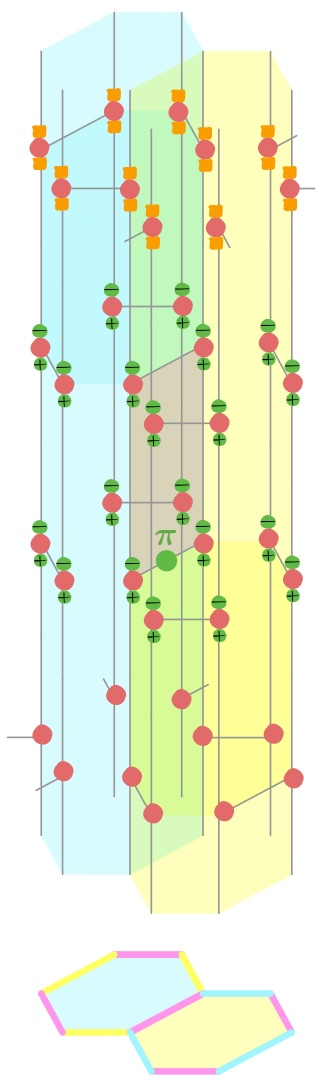
\includegraphics[height=200pt]{figures/repeating_measurements/repeated_DCCC_ordinary_edge_measurement_error_a}
        \caption{}
        \label{fig:repeated_DCCC_ordinary_edge_measurement_error_a}
    \end{subfigure}
    \begin{subfigure}[c]{0.18\textwidth}
        \centering
        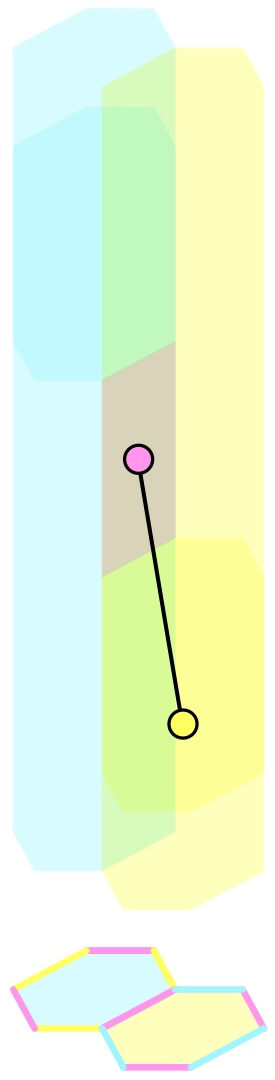
\includegraphics[height=200pt]{figures/repeating_measurements/repeated_DCCC_ordinary_edge_measurement_error_b}
        \caption{}
        \label{fig:repeated_DCCC_ordinary_edge_measurement_error_b}
    \end{subfigure}
    \begin{subfigure}[c]{0.14\textwidth}
        \centering
        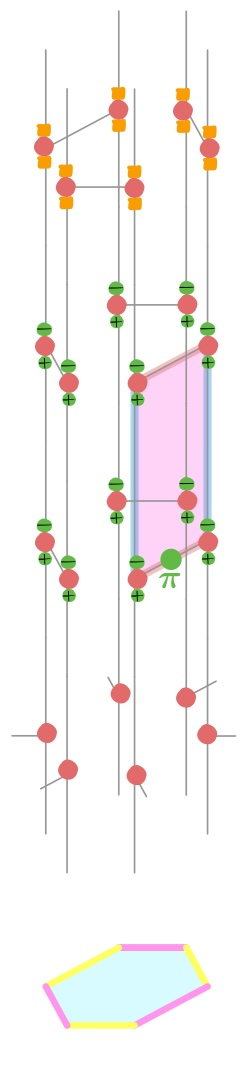
\includegraphics[height=200pt]{figures/repeating_measurements/repeated_DCCC_ordinary_edge_measurement_error_c}
        \caption{}
        \label{fig:repeated_DCCC_ordinary_edge_measurement_error_c}
    \end{subfigure}
    \begin{subfigure}[c]{0.14\textwidth}
        \centering
        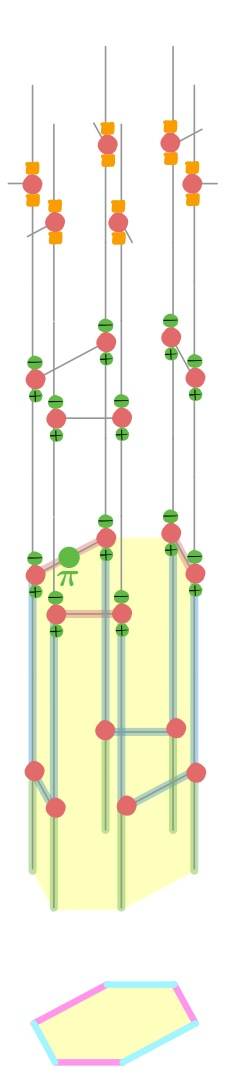
\includegraphics[height=200pt]{figures/repeating_measurements/repeated_DCCC_ordinary_edge_measurement_error_d}
        \caption{}
        \label{fig:repeated_DCCC_ordinary_edge_measurement_error_d}
    \end{subfigure}
    \begin{subfigure}[c]{0.14\textwidth}
        \centering
        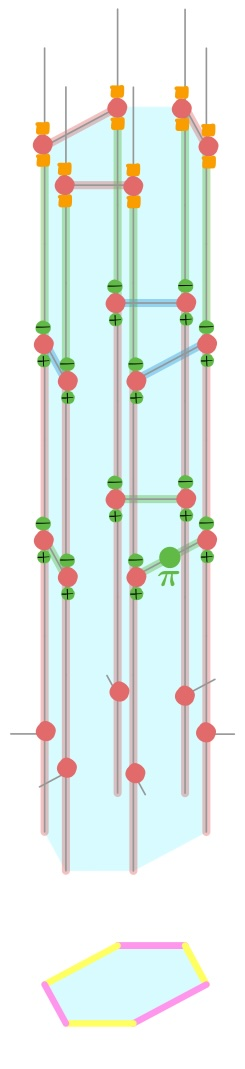
\includegraphics[height=200pt]{figures/repeating_measurements/repeated_DCCC_ordinary_edge_measurement_error_e}
        \caption{}
        \label{fig:repeated_DCCC_ordinary_edge_measurement_error_e}
    \end{subfigure}
    \begin{subfigure}[c]{0.14\textwidth}
        \centering
        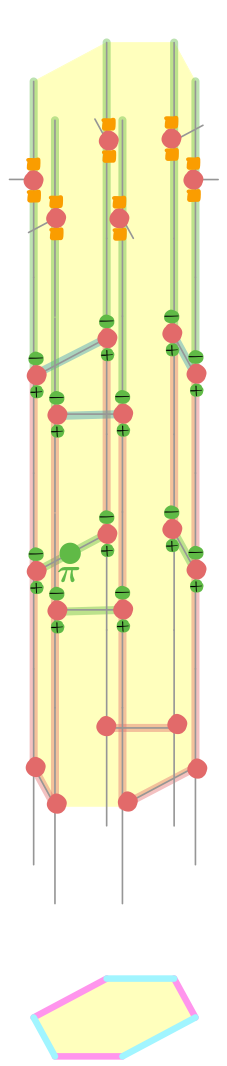
\includegraphics[height=200pt]{figures/repeating_measurements/repeated_DCCC_ordinary_edge_measurement_error_f}
        \caption{}
        \label{fig:repeated_DCCC_ordinary_edge_measurement_error_f}
    \end{subfigure}
    \caption{
        \textbf{(a)} A measurement error in the $X^2 Y^2 Z^2$ code.
        \textbf{(b)} The ordinary edge it corresponds to in the decoding graph.
        \textbf{(c, d)} The $E$ detectors the error violates, drawn as Pauli webs.
        \textbf{(e, f)} The $M$ detectors the error sits on but does not violate, drawn as Pauli webs.
        Compare this figure with \Cref{fig:XYZ_measurement_error}, where an analogous error in the $X^1 Y^1 Z^1$ code corresponded to a hyperedge in the decoding graph.
        This would still have been the case in the $X^2 Y^2 Z^2$ code had the measurement error occurred in the last of the $r=2$ repeated rounds of measurements.
        But for all other rounds such an error now corresponds to an ordinary edge.
        In general, repeating measurements reduces the number of measurement errors corresponding to hyperedges, which would suggest a plateau in the improvement from using belief matching over MWPM (\Cref{dif:repeated_meas_errors_hyperedges}), and indeed this seems to be the case numerically (\Cref{fig:XaYbZc_teraquop_volumes_measurement_bias}).
    }
    \label{fig:repeated_DCCC_ordinary_edge_measurement_error}

    \vspace{20pt}

    \begingroup
    \renewcommand*{\arraystretch}{1.2}
        \centering
        \begin{tabular}{|r|c|c|c|c|c|c|}
            \hline
            & \multicolumn{3}{c|}{$X^r Y^r Z^r$} & \multicolumn{3}{c|}{$X^r Z^r$} \\
            \hline
            & \makecell{Direct parity \\ meas.} & \makecell{Meas.\\noise} & \makecell{Z noise} & \makecell{Direct parity \\ meas.} & \makecell{Meas.\\noise} & \makecell{Z noise} \\
            \hline
            $d_{s, E}$ & $n_E$ & $r n_E \to \infty$ & $n_E$ & $n_E$ & $r n_E \to \infty$ & $n_E$ \\
            \hline
            $d_{s, M}$ & $\frac{4}{3}n_M$ & $r \frac{4}{3}n_M \to \infty$ & $\frac{4}{3}n_{M}$ & $\frac{4}{3}n_M$ & $r \frac{4}{3}n_M \to \infty$ & $\infty$ \\
            \hline
            $d_{t, E}$ & $\frac{h_\mathbf{r}}{2r} \to 0$ & $\frac{h_\mathbf{r}}{2}$ & $\frac{h_\mathbf{r}}{2r} \to 0$ & $\min\{\frac{h_\mathbf{r}}{2r}, \frac{h_\mathbf{r}}{4}\} \to 0$ & $\frac{h_\mathbf{r}}{4}$ & $\frac{h_\mathbf{r}}{2r} \to 0$ \\
            \hline
            $d_{t, M}$ & $\frac{h_\mathbf{r}}{2r} \to 0$ & $\frac{h_\mathbf{r}}{2}$ & $\frac{h_\mathbf{r}}{2r} \to 0$ & $\min\{\frac{h_\mathbf{r}}{2r}, \frac{h_\mathbf{r}}{4}\} \to 0$ & $\frac{h_\mathbf{r}}{4}$ & $\infty$ \\
            \hline
            $p_h$ & $\frac{2}{9} + \frac{1}{3r} \to \frac{2}{9}$& $\frac{1}{r} \to 0$ & $\frac{1}{3}$ & $\frac{2}{9}$ & $0$ & $0$ \\
            \hline
        \end{tabular}
        \captionof{table}{
            Comparison of the $X^r Y^r Z^r$ and $X^r Z^r$ codes, for $r > 1$.
            The first four rows show the spacelike $E$ and $M$ distances and timelike $E$ and $M$ distances respectively.
            The final row shows the hyperedge likelihood.
            The arrows denote the limit of an expression as $r$ tends to infinity.
            Repeating measurements increases the spacelike distances under pure measurement noise (\Cref{dif:repeated_spacelike_logicals}),
            but decreases the timelike distances under pure data qubit noise (\Cref{dif:repeated_timelike_logicals}).
            One might expect this to be reflected in the teraquop widths, lengths and heights, but the simulation results show this isn't the case (\Cref{fig:X1Z1_X3Z3_comparison}).
            Repeating measurements also decreases the frequency with which measurement errors correspond to hyperedges in the decoding graph.
            This explains why the improvement given by decoding with belief matching rather than MWPM plateaus the more we repeat measurements (\Cref{fig:XaYbZc_teraquop_volumes_measurement_bias}).
        }
        \label{tab:repeated_xyz_css_distances}
\endgroup
\end{figure}


\begin{figure}[p]
    \centering
    \begin{subfigure}[b]{0.24\textwidth}
        \centering
        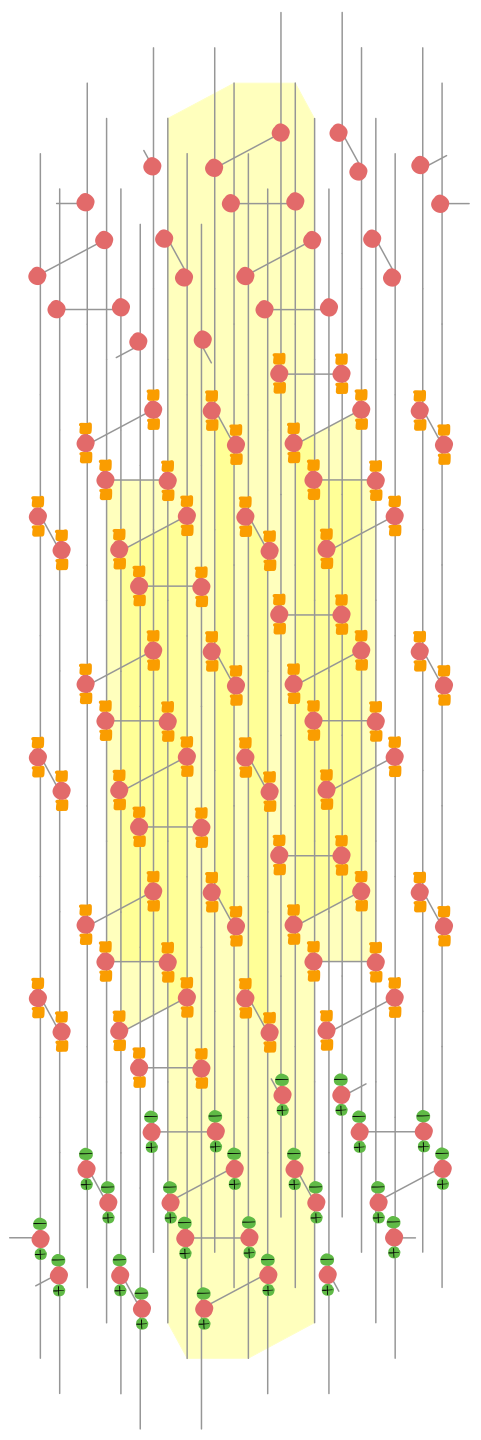
\includegraphics[height=330pt]{figures/repeating_measurements/face_detector_neighbourhood_web.png}
        \caption{}
        \label{fig:ZX_plus_init}
    \end{subfigure}
    \begin{subfigure}[b]{0.24\textwidth}
        \centering
        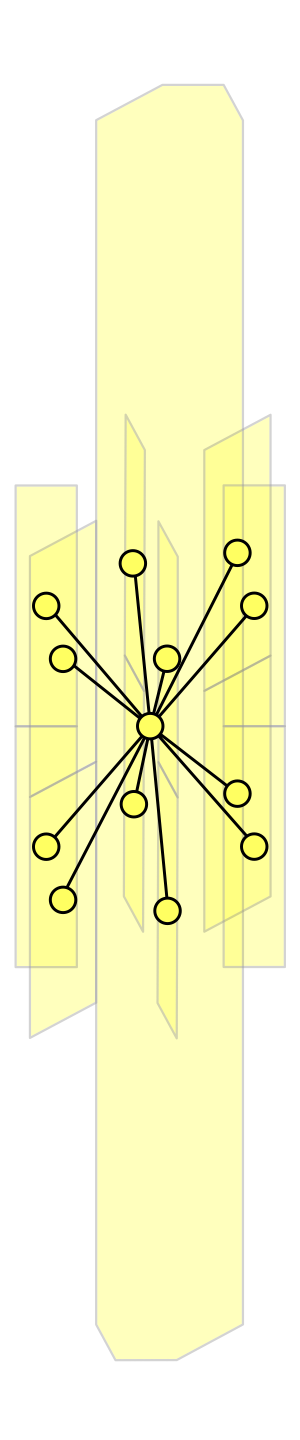
\includegraphics[height=330pt]{figures/repeating_measurements/face_detector_neighbourhood_graph.png}
        \caption{}
        \label{fig:ZX_X_meas}
    \end{subfigure}
    \begin{subfigure}[b]{0.24\textwidth}
        \centering
        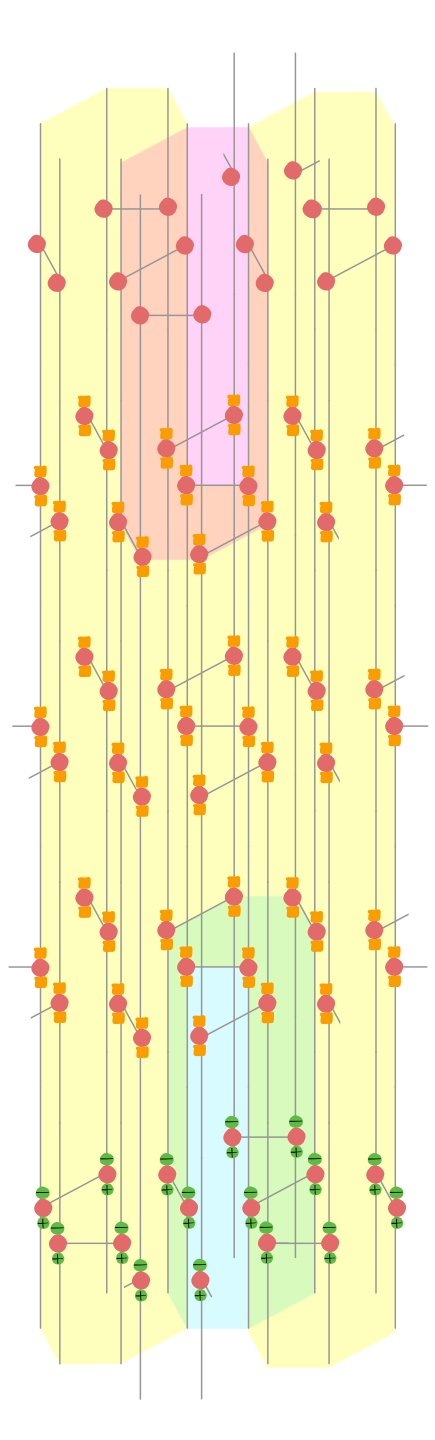
\includegraphics[height=330pt]{figures/repeating_measurements/edge_detector_neighbourhood_web.png}
        \caption{}
        \label{fig:ZX_CNOT}
    \end{subfigure}
    \begin{subfigure}[b]{0.24\textwidth}
        \centering
        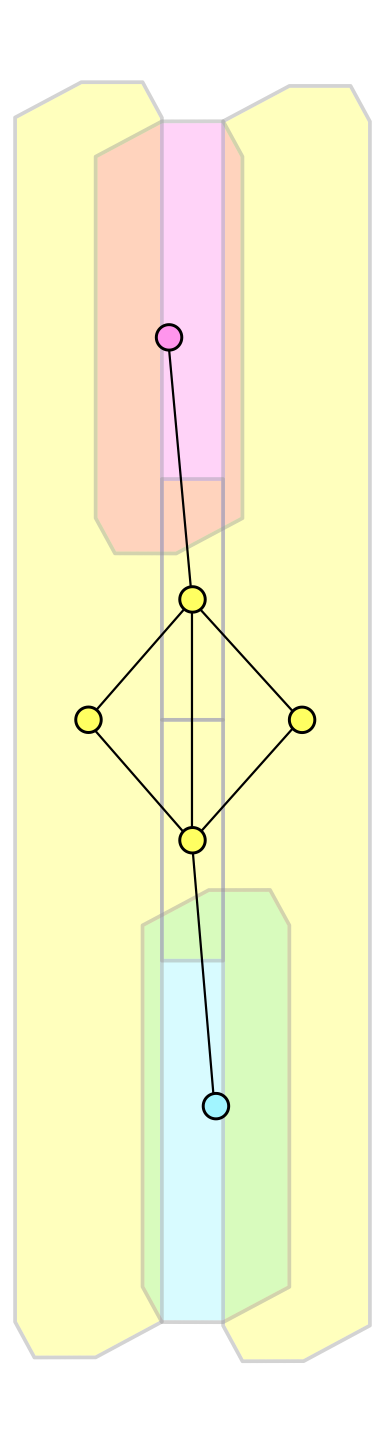
\includegraphics[height=330pt]{figures/repeating_measurements/edge_detector_neighbourhood_graph.png}
        \caption{}
        \label{fig:ZX_XX_meas_circuit_YZ_error}
    \end{subfigure}
    \caption{
        \textbf{(a)} Five timesteps of the $X^3 Y^3 Z^3$ code, centered on a yellow face.
        The shaded yellow areas denote a face detector and 12 edge detectors.
        \textbf{(b)} The edges between the face detector and the 12 edge detectors in the decoding graph.
        The face detector has 12 further edges (unshown) to other detectors in the ordinary decoding graph, exactly analogous to the 12 edges it has in $\Cref{fig:decoding_graph_face_detector_neighbourhood}$ in the $X^1 Y^1 Z^1$ code.
        So altogether it now has 24 edges.
        \textbf{(c)} The same five timesteps of the $X^3 Y^3 Z^3$ code, but now centered on a yellow edge, with shaded areas indicating detectors.
        \textbf{(d)} The neighbourhoods of the two edge detectors in the ordinary decoding graph.
        Note each has degree 4.
        All of the above holds more generally, in that in the ordinary decoding graph for each $X^a Y^b Z^c$ and $X^a Z^b$ code, every edge detector will have degree 4, and every face detector will have degree $12 + 6(r-1)$, where $r$ is the number of repeated measurement rounds for the edges in consideration (here $r=3$).
        So repeating measurements generally increases the maximum vertex degree but reduces the average vertex degree in the decoding graph (\Cref{tab:repeated_xyz_css_averages}).
        The former suggests a general decrease in performance while the latter suggests an increase.
    }
    \label{fig:repeated_decoding_graph_neighbourhoods}
\end{figure}

The other key difference pertains to vertex degrees in a DCCC's decoding graph.
The degree of vertices in a code's decomposed decoding graph in general affects decoding performance; the lower the better~\cite{OscarSubsystemGaugeFixing}.
In any unrepeated DCCC, we said every vertex (i.e.\ detector) has degree 12 (\Cref{fig:decoding_graph_face_detector_neighbourhood}).
Repeating measurements introduces edge detectors, whose corresponding vertices always have degree 4 (\Cref{fig:repeated_decoding_graph_neighbourhoods}),
but it also increases the degree of the vertices corresponding to face detectors.
For the $X^a Y^b Z^c$ and $X^a Z^b$ codes this is overall a positive change,
in the sense that the average vertex degree in the decomposed decoding graph tends from 12 down to 6 as the number of repeated measurements increases.

\begin{difference}\label{dif:repeating_decoding_graph_degrees}
    Repeating measurements decreases the average vertex degree in the decoding graph of a DCCC.
\end{difference}

This difference would seem to predict a general performance increase for repeated DCCCs versus their unrepeated counterparts.

% \begingroup
% \renewcommand*{\arraystretch}{1.5}
% \begin{table}[htbp]
%     \centering
%     \begin{tabular}{|r|c|c|c|c|c|c|}
%         \hline
%         & \multicolumn{3}{c|}{$X^r Y^r Z^r$} & \multicolumn{3}{c|}{$X^r Z^r$} \\
%         \hline
%         & \makecell{Phenom. \\ noise} & \makecell{Meas.\\noise} & \makecell{Z noise} & \makecell{Phenom. \\ noise} & \makecell{Meas.\\noise} & \makecell{Z noise} \\
%         \hline
%         $d_{s, E}$ & $n_E$ & $r n_E \to \infty$ & $n_E$ & $n_E$ & $r n_E \to \infty$ & $n_E$ \\
%         \hline
%         $d_{s, M}$ & $\frac{4}{3}n_M$ & $r \frac{4}{3}n_M \to \infty$ & $\frac{4}{3}n_{M}$ & $\frac{4}{3}n_M$ & $r \frac{4}{3}n_M \to \infty$ & $\infty$ \\
%         \hline
%         $d_{t, E}$ & $\frac{h_\mathbf{r}}{2r} \to 0$ & $\frac{h_\mathbf{r}}{2}$ & $\frac{h_\mathbf{r}}{2r} \to 0$ & $\min\{\frac{h_\mathbf{r}}{2r}, \frac{h_\mathbf{r}}{4}\} \to 0$ & $\frac{h_\mathbf{r}}{4}$ & $\frac{h_\mathbf{r}}{2r} \to 0$ \\
%         \hline
%         $d_{t, M}$ & $\frac{h_\mathbf{r}}{2r} \to 0$ & $\frac{h_\mathbf{r}}{2}$ & $\frac{h_\mathbf{r}}{2r} \to 0$ & $\min\{\frac{h_\mathbf{r}}{2r}, \frac{h_\mathbf{r}}{4}\} \to 0$ & $\frac{h_\mathbf{r}}{4}$ & $\infty$ \\
%         \hline
%         $p_h$ & $\frac{2}{9} + \frac{1}{3r} \to \frac{2}{9}$& $\frac{1}{r} \to 0$ & $\frac{1}{3}$ & $\frac{2}{9}$ & $0$ & $0$ \\
%         \hline
%     \end{tabular}
%     \caption{
%         Comparison of the $X^r Y^r Z^r$ and $X^r Z^r$ codes, for $r > 1$.
%         The first four rows show the spacelike $E$ and $M$ distances and timelike $E$ and $M$ distances respectively.
%         The final row shows the hyperedge likelihood.
%         The arrows denote the limit of an expression as $r$ tends to infinity.
%         Repeating measurements increases the spacelike distances under pure measurement noise (\Cref{dif:repeated_spacelike_logicals}),
%         but decreases the timelike distances under pure data qubit noise (\Cref{dif:repeated_timelike_logicals}).
%         One might expect this to be reflected in the teraquop widths, lengths and heights, but the simulation results show this isn't the case (\Cref{fig:X1Z1_X3Z3_comparison}).
%         Repeating measurements also decreases the frequency with which measurement errors correspond to hyperedges in the decoding graph.
%         This explains why the improvement given by decoding with belief matching rather than MWPM plateaus the more we repeat measurements (\Cref{fig:XaYbZc_teraquop_volumes_measurement_bias}).
%     }
%     \label{tab:repeated_xyz_css_distances}
% \end{table}
% \endgroup

\subsection{Direct parity measurement noise results}\label{subsec:repeating_measurements_direct_parity_measurement_noise}

\Cref{fig:phenomenological_noise_volume_plot_pymatching,fig:phenomenological_noise_volume_plot_beliefmatching} show the teraquop volumes of the best $X^a Y^b Z^c$ and $X^a Z^b$ codes under direct parity measurement noise models of different biases, decoded with MWPM and belief matching respectively.

\begin{keypoint}
    Repeating measurements improves the teraquop volumes of both codes under both decoders when the noise is measurement-biased, but otherwise it has a negligible effect.
\end{keypoint}

One can see this most clearly by looking at the hearts ($\heartsuit$) subplot in \Cref{fig:phenomenological_noise_volume_plot_pymatching,fig:phenomenological_noise_volume_plot_beliefmatching};
under MWPM (\Cref{fig:phenomenological_noise_volume_plot_pymatching}) all but one of the ten best codes involve repeating measurements in some way,
and under belief matching (\Cref{fig:phenomenological_noise_volume_plot_beliefmatching}) it's all ten.
This chimes with the intuition that repeating measurements gives us more confidence about faulty measurements.
At the same time it seems to contradict the intuition that repeating measurements might improve performance in general (\Cref{dif:repeating_detectors,dif:repeating_decoding_graph_degrees}), and particularly in the case of $Z$-biased noise by spending more time measuring certain operators (\Cref{dif:repeating_asymmetric_schedule}). That said, we only tested a $Z$-noise bias of up to $\eta_Z = 16$, whereas in other work orders of magnitude higher values are considered -- e.g. bias of up to $\eta_Z = 10^6$ is considered in \Ccite{Chamberland_2022}.

\subsection{Auxiliary qubit circuit noise results}\label{subsec:repeating_measurements_auxiliary_qubit_circuit_noise}

\Cref{fig:pymatching_circuit_level_noise_volume_plot,fig:beliefmatching_circuit_level_noise_volume_plot} show the teraquop volumes of the best codes under the three auxiliary qubit circuit noise models, decoded with MWPM and belief matching respectively.
In all three cases, there is not much to be gained from repeating measurements.
Perhaps the only exception is that in the belief matching case under the EM3 noise model, the $X^2 Z^2$ code has a noticeably better teraquop volume than the $X^1 Z^1$ code.
But both are outperformed by the $X^1 Y^1 Z^1$ code, which has the best teraquop footprint out of all the codes in this regime.

%The bottom two subfigures in \Cref{fig:repeated_measurements_timelike_distances} show the timelike distances of the various $X^a Y^b Z^c$ and $X^a Z^b$ codes under circuit-level noise.
%While there's a lot going on, perhaps the main thing to notice is that the timelike distances of the $X^a Z^b$ codes are unchanged regardless of the noise model used, whereas the timelike distances of the $X^a Y^b Z^c$ codes are in general reduced when moving to either circuit-level noise model.

\begin{figure}[t]
    \centering
    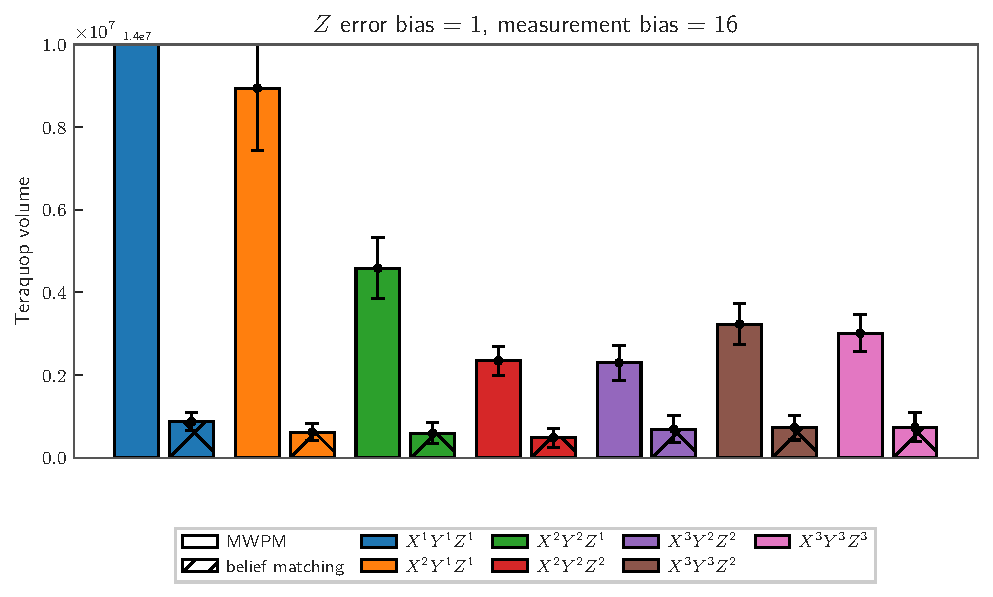
\includegraphics[width=\linewidth]{figures/repeating_measurements/X1Y1Z1_X2Y2Z2_X3Y3Z3_comparison.pdf}
    \caption{
        Teraquop volumes of the $X^aY^bZ^c$ code for direct parity measurement noise with measurement bias 16,
        and an increasing number $a + b + c$ of repeated rounds of measurements.
        As predicted by \Cref{dif:repeated_meas_errors_hyperedges}, using belief matching rather than MWPM initially makes a huge difference to the volume, but this plateaus the more we repeat measurements.
    }
    \label{fig:XaYbZc_teraquop_volumes_measurement_bias}
\end{figure}

\begin{figure}[p]
    \centering
    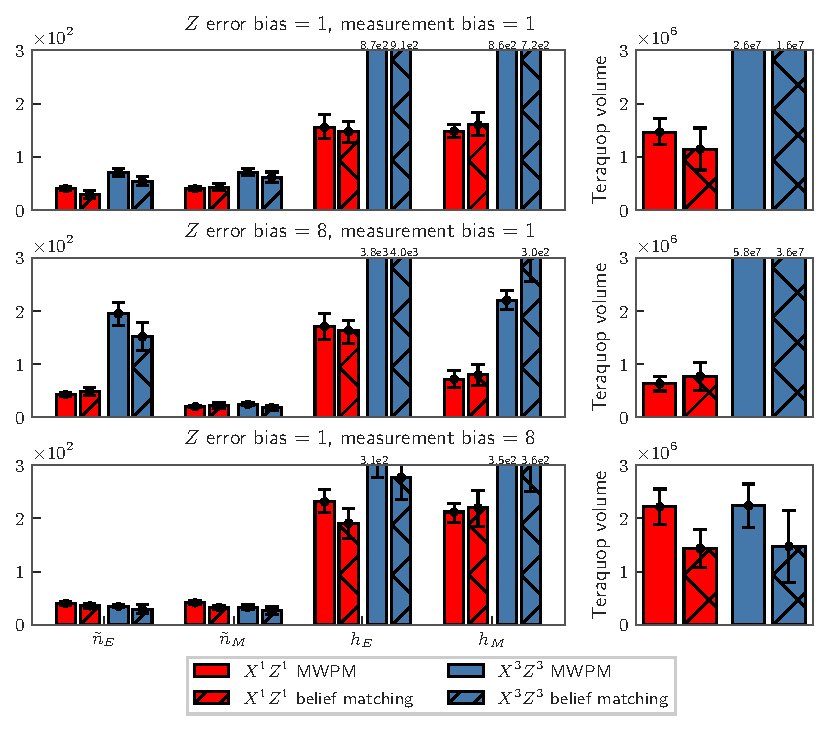
\includegraphics[width=\linewidth]{figures/repeating_measurements/X1Z1_X3Z3_comparison}
    \caption{
        Comparison of $\tilde{n}_E, \tilde{n}_M, \tilde{h}_E, \tilde{h}_M,$ and teraquop volume of the $X^1Z^1$ and $X^3Z^3$ code decoded using MWPM and belief matching for unbiased, $Z$-biased, and measurement-biased direct parity measurement noise.
        Based on \Cref{dif:repeated_spacelike_logicals}, we expected that repeating measurements would reduce the teraquop width and length $\tilde{n}_E$ and $\tilde{n}_M$, especially in the case of measurement-biased noise.
        Similarly, based on \Cref{dif:repeated_timelike_logicals}, we expected that repeating measurements would increase the teraquop heights $\tilde{h}_E$ and $\tilde{h}_M$, especially in the case of $Z$-biased noise.
        Neither of these predictions are borne out by the simulation results here.
        In no cases does repeating measurements significantly reduce the teraquop width or length,
        and while it's true that repeating measurements increases the teraquop heights, the fact that this increase is greatest for unbiased noise suggests the cause is something more than \Cref{dif:repeated_timelike_logicals}.
    }
    \label{fig:X1Z1_X3Z3_comparison}
\end{figure}

\begin{figure}[p]
    \centering
    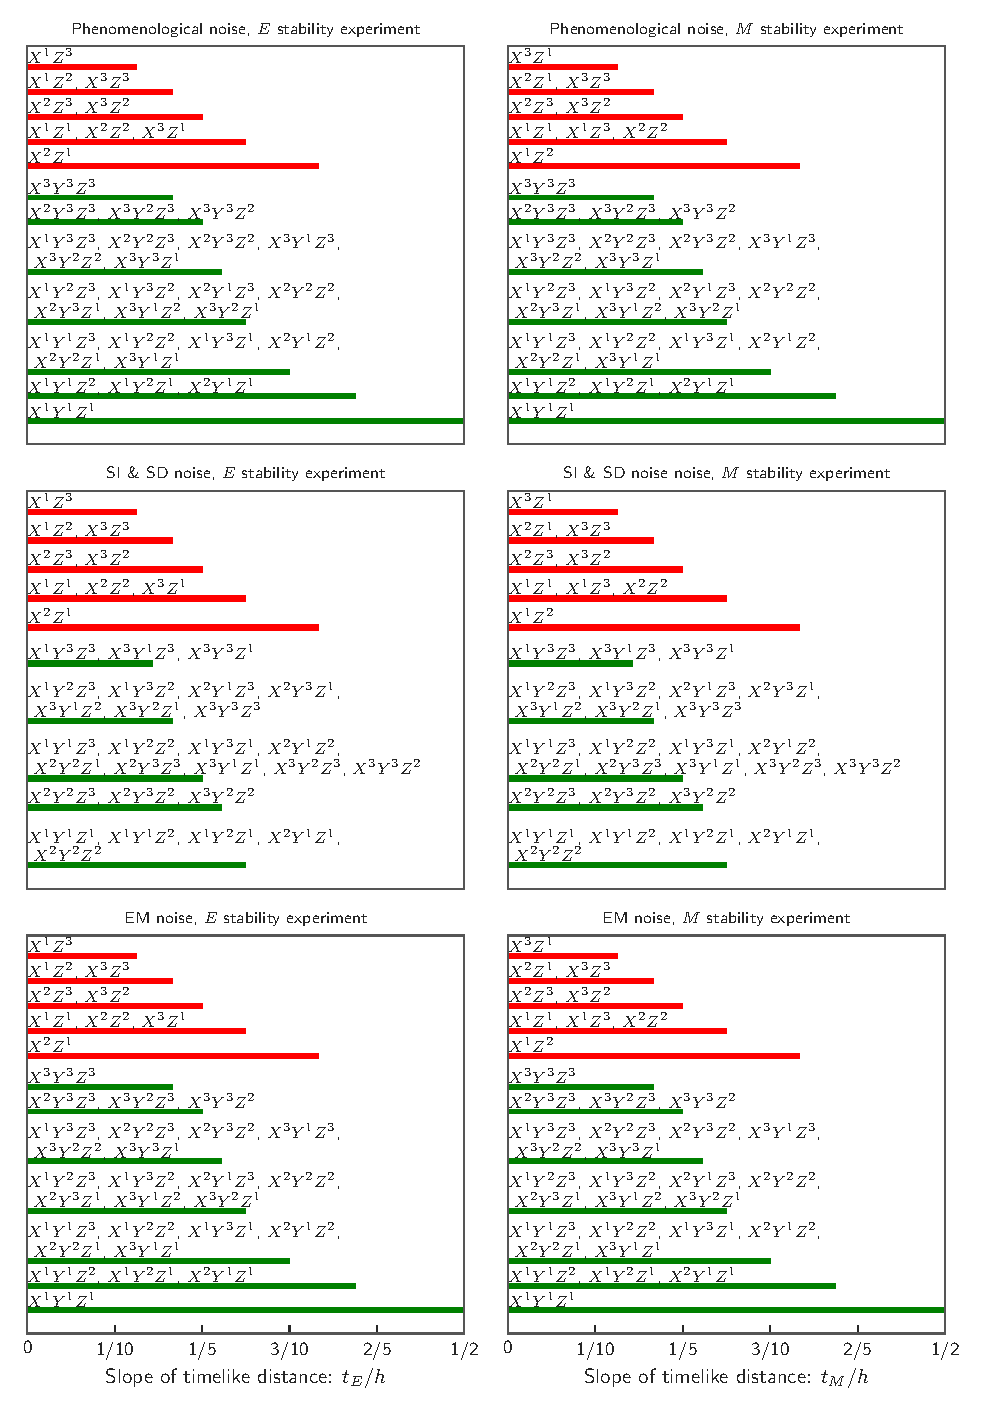
\includegraphics[width=0.9\linewidth]{figures/repeating_measurements/timelike_distance.pdf}
    \caption{
        Plots showing the timelike distances of $(n_E, n_M, h)$-blocks of $X^a Y^b Z^c$ and $X^a Z^b$ codes under different noise models as a fraction of the block height $h$.
        Since standard depolarizing noise and superconducting-inspired noise differ only in the probabilites of the certain gates occurring, and not in which gates can occur, any notions of distance are identical across both models.
        So we bundle these models together into a `single-qubit measurements' noise model (middle row).
        One can see that the $X^a Z^b$ code timelike distances are unchanged across all three noise models.
        The timelike distances of $X^a Y^b Z^c$ codes are in general reduced under single-qubit measurements noise as compared to direct parity measurement noise,
        but preserved under entangling measurements noise.
        This feature doesn't seem to be significant enough to appear in the simulation results -- e.g.\ in \Cref{fig:beliefmatching_circuit_level_noise_volume_plot}, under the two single-qubit measurements noise models the $X^1 Y^1 Z^1$ code still has the best teraquop volume.
    }
    \label{fig:repeated_measurements_timelike_distances}
\end{figure}
